%
% projektion.tex
%
% (c) 2018 Prof Dr Andreas Müller, Hochschule Rapperswil
%
\documentclass[tikz]{standalone}
\usepackage{times}
\usepackage{amsmath}
\usepackage{txfonts}
\usepackage[utf8]{inputenc}
\usepackage{graphics}
\usetikzlibrary{arrows,intersections,math}
\begin{document}

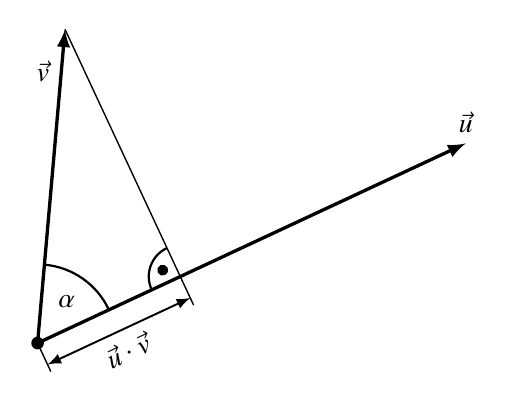
\begin{tikzpicture}[>=latex,thick]

\begin{scope}[rotate=25]

\def\a{60}
\def\l{4}
\def\r{1}

% Vektor u
\draw[->,line width=1.2pt] (0,0)--(6,0);
\node at (6,0) [above] {$\vec{u}$};

% Vektor v
\draw[->,line width=1.2pt] (0,0)--({\l*cos(\a)},{\l*sin(\a)});
\node at ({0.8*\l*cos(\a)},{0.8*\l*sin(\a)}) [above left] {$\vec{v}$};

% Projektion
\draw[line width=0.5pt] ({\l*cos(\a)},{\l*sin(\a)})--({\l*cos(\a)},-0.4);
\draw[line width=0.5pt] (0,0)--(0,-0.4);

% rechter Winkel
\def\rr{0.4}
\draw (2,\rr) arc (90:180:\rr);
\fill ({2-0.42*\rr},{0.42*\rr}) circle[radius=0.07];

% Winkel alpha
\draw (\r,0) arc (0:\a:\r);
\node at ({0.65*\r*cos(\a/2)},{0.65*\r*sin(\a/2)}) {$\alpha$};

% Bemassung
\draw[<->,line width=0.7pt] (0,-0.3)--({\l*cos(\a)},-0.3);
\node at ({0.5*\l*cos(\a)},-0.3) [below,rotate=25] {$\vec{u}\cdot\vec{v}$};

% Nullunkt
\fill (0,0) circle[radius=0.08];

\end{scope}

\end{tikzpicture}

\end{document}

